

\chapter{Методы и их применение} \label{chap2}

\section{Имитация отжига}

\noindent
\textit{Имитация отжига} (simulated annealing) представляет собой алгоритм решения задачи по поиску глобального оптимума некоторой функции~$F:$~$\mathbb{X} \to \mathbb{R}$ через упорядоченный стохастический поиск, базирующийся на моделировании физического процесса кристализации вещества из жидкого состояние в твердое.

Для описания метода рассмотрим задачу нахождения глобального минимума:
\[
	F(x) \to \min \limits _{x \in \mathbb{X}},
\]

\noindent где~$x = (x_{1},\ldots , x_{m})$~--- вектор всех состояний, $\mathbb{X}$~--- множество всех состояний.

\subsection{Алгоритм}

\noindent Положим, что~$k = 0$~и изначально температура зафиксированна на определенном уровне~$T(k) = const$.


\begin{enumerate}
	\item  Из множества всех состояний выберем случайный элемент~$\widehat{x}(k) \equiv x_i$,

	$i \in (1, ..., m)$.

	\item Понизим температуру одним из следующих способов:

		\begin{enumerate}
			\item Больцмановский отжиг
			\begin{equation}
			T(k) =  \dfrac{T(0)}{\ln (1 + k)}, \ k > 0
			\label{eq:boltzman}
			\end{equation}

			\item Отжиг Коши
			\begin{equation}
			T(k)  =  \dfrac{T(0)}{k}
			\end{equation}

			\item Метод тушения
			\begin{equation}
			T(k+1) = \alpha T(k),\ \alpha \in (0, 1)
			\end{equation}

		\end{enumerate}


	\item Пусть следующий элемент зависит от функции из семейства симметричных вероятностных распределений $G:$~$ \mathbb{X} \to \mathbb{X}$, порождающей новое состояние:
	\[
	\tilde{x}(k) \thicksim G(\widehat{x}(k), T(k)).
	\]

	\begin{enumerate}

		\item Часто G выбирается из семейства нормальных распределений:
		\begin{equation}
		\label{eq:normal_G}
		G(\tilde{x}; \widehat{x}, T)
		=
		\dfrac{1}
		{\sqrt{(2\pi)^{D} T}}
		\exp
		\left\lbrace
		\dfrac{- |\tilde{x} - \widehat{x}|^2}{2T}
		\right\rbrace,
		\end{equation}

		где $\widehat{x}$ — математическое ожидание, $T$  — дисперсия, $D$ — размерность пространства всех состояний.

		\item Также для D = 1 используется распределение Коши с плотностью:
		\begin{equation}
		G(\tilde{x}; \widehat{x}, T)
		=
		\dfrac{1}{\pi}
		\dfrac{T}{|\tilde{x}- \widehat{x}|^2 + T^2},
		\end{equation}

		где~$\widehat{x}$~--- параметр сдвига, $T$~--- параметр масштаба.





	\end{enumerate}

	\item Рассчитываем разницу двух функций:
	\[
	\Delta F =
	F(\tilde{x}(k))
	-
	F(\widehat{x}(k)).
	\]

	\item Принимаем~$\tilde{x}(k)$~за новый элемент, то есть~$\widehat{x}(k+1) \equiv \tilde{x}(k)$, с вероятностью
	\begin{equation}
	\mathbb{P}(\{\widehat{x}(k+1) = \tilde{x}(k)\})
	=
	\begin{cases}
	1,
	&
	\Delta F <0
	\\
	\exp
	\left\lbrace
	- \dfrac {\Delta F}{T(k)}
	\right\rbrace ,
	&
	\Delta F \geqslant 0
	\end{cases}
	\end{equation}

	и отвергаем его, то есть~$\widehat{x}(k+1) \equiv \widehat{x}(k)$, с вероятностью
	\[
	q
	=
	1 - \mathbb{P}(\{\widehat{x}(k+1) = \tilde{x}(k)\}).
	\]

	Заметим, чем выше температура, тем больше вероятность принять состояние хуже текущего ($\Delta F \geqslant 0$).

	\item Возвращаемся к пункту 2, пока не достигнем глобального минимума.

\end{enumerate}


%%%%%%%%%%%%%%%%%%%%%%%%%%%%%%%%%%%%%%%%%%%%%%%%%%%%%%%%


\subsection{N ферзей}
\noindent Рассмотрим задачу, в которой необходимо расставить $N$ ферзей на шахматной доске размера $N \times  N$ так, чтобы ни один из них не <<бил>> другого.

В таком случае, множество всех состояний $\mathbb{X}$ будет содержать всевозможные расстановки ферзей на шахмотной доске. Общее число возможных расположений $n$ ферзей на $N \times N$-клеточной доске равно:
\[
{\begin{pmatrix} N \times N  \\ n \end{pmatrix}} = \dfrac{N \times N!}{n! (N \times N - n)!}
\]

Тогда  функция~$F:$~$\mathbb{X} \to \mathbb{R}$ будет выдавать количество атак ферзей, и решением данной задачи будет нахождение такого распложения~$x^{*}$, что~$F(x^*) \equiv 0$.

Зафиксируем изначальное расположение ферзей на шахматной доске. Очевидно, что несколько ферзей не могут находиться на одной вертикали или горизонтали, ибо тогда они будут находиться под ударом друг-друга. Следовательно, наша задача сужается к поиску расположения:
\begin{equation}
x* = (q_1, ..., q_n) = \{(1, h_1), ..., (n, h_n)\}, h_1 \neq ...  \neq h_n,
\end{equation}

где $(i, h_i)$ — расположение ферзя $q_i$ на i-ой вертикали по горизонтали $h_i$.

Отметим, что такая задача имеет $N!$ решений.

\newgame
\fenboard{q7/1q6/2q5/3q4/4q3/5q2/6q1/7q w - - 0 1}

\begin{figure}[h!]
	\begin{center}
		\showboard
		\legend{}
		\caption{ --- Изначальное расположение.}
		\label{img:nonopt}
	\end{center}
\end{figure}

Определим функцию, которая будет создавать изначальное неоптимальное расположение, в общем виде. Учитем, что несколько ферзей не могут находиться на одной вертикали или горизонтали.

\begin{pyin}
def queens(N):
  ver = np.arange(1, N + 1)
  hor = np.arange(1, N + 1)
  np.random.shuffle(hor)
  return np.column_stack((ver, hor)) # получаем массив
  # размерности (N, 2), отождествляющий расположение ферзей
\end{pyin}

Выведем первоначальное расположение ферзей для стандартной доски $8 \times 8$, где первый столбец массива — расположение по вертикали, второй столбец массива — расположение по горизонтали. Для наглядности — презентации оптимизационного процесса — выстроим изначальную расстановку на главной диагонали (рис. \ref{img:nonopt}).


\begin{pyin}
matrix = queens(8)
matrix
\end{pyin}

\begin{pyout}
array([[1, 1],
       [2, 2],
       [3, 3],
       [4, 4],
       [5, 5],
       [6, 6],
       [7, 7],
       [8, 8]])
\end{pyout}


Функция F, которая выявляет количество атак ферзей, выглядит следующим образом:
\begin{pyin}
def F(Q, N):
  cnt = 0
  for i in range(N):
     for j in range(i + 1, N):
         if abs(Q[i, 0] - Q[j, 0]) == abs(Q[i, 1] - Q[j, 1]):
             cnt += 1
  return cnt * 2 # учитываем взаимные атаки
\end{pyin}

Посмотрим, сколько у атак у исходной расстановки.
\begin{pyin}
F(matrix, 8)
\end{pyin}

\begin{pyout}
56
\end{pyout}

В нашей задачи функция G будет случайной незначительной перестановкой номеров горизонтали в исходном наборе.

\begin{pyin}
def G(Q, N):
  pos = Q.copy()
  while True:
     i = np.random.randint(0, N - 1)
     j = np.random.randint(0, N - 1)
     if i != j:
        break
  pos[i, 1], pos[j, 1] = pos[j, 1], pos[i, 1]
  return pos # получаем новое расположение
\end{pyin}

Теперь выведем и сам метод имитации отжига.

\begin{pyin}
def SA(Q, T, schedule):
  N = np.shape(Q)[0]
  x_hat = Q.copy()
  while F(x_hat, N) != 0:
     x_tilda = G(x_hat, N)
     delta = F(x_tilda, N) - F(x_hat, N)
     prob = np.exp(- delta / T)
\end{pyin}

\begin{pyprint}
     if (delta < 0) or (prob >= np.random.random()):
        x_hat = x_tilda
     T *= schedule # используем метод тушения для понижения температуры
  return x_hat
\end{pyprint}


\newgame
\fenboard{2q5/4q3/1q6/7q/q7/6q1/3q4/5q2 w - - 0 1}

\begin{figure}[h!]
	\begin{center}
		\showboard
		\legend{}
		\caption[р]{ --- Оптимальное расположение}
		\label{img:opt}
	\end{center}
\end{figure}


Так для нашего примера с гиперпараметрами $T(0) = 100, \alpha = 0.9$ мы получаем следующее оптимальное решение (рис. \ref{img:opt}):

\begin{pyin}
SA(matrix, 100, 0.9)
\end{pyin}

\begin{pyout}
array([[1, 4],
       [2, 6],
       [3, 8],
       [4, 2],
       [5, 7],
       [6, 1],
       [7, 3],
       [8, 5]])
\end{pyout}

\begin{figure}[h!]
\centering
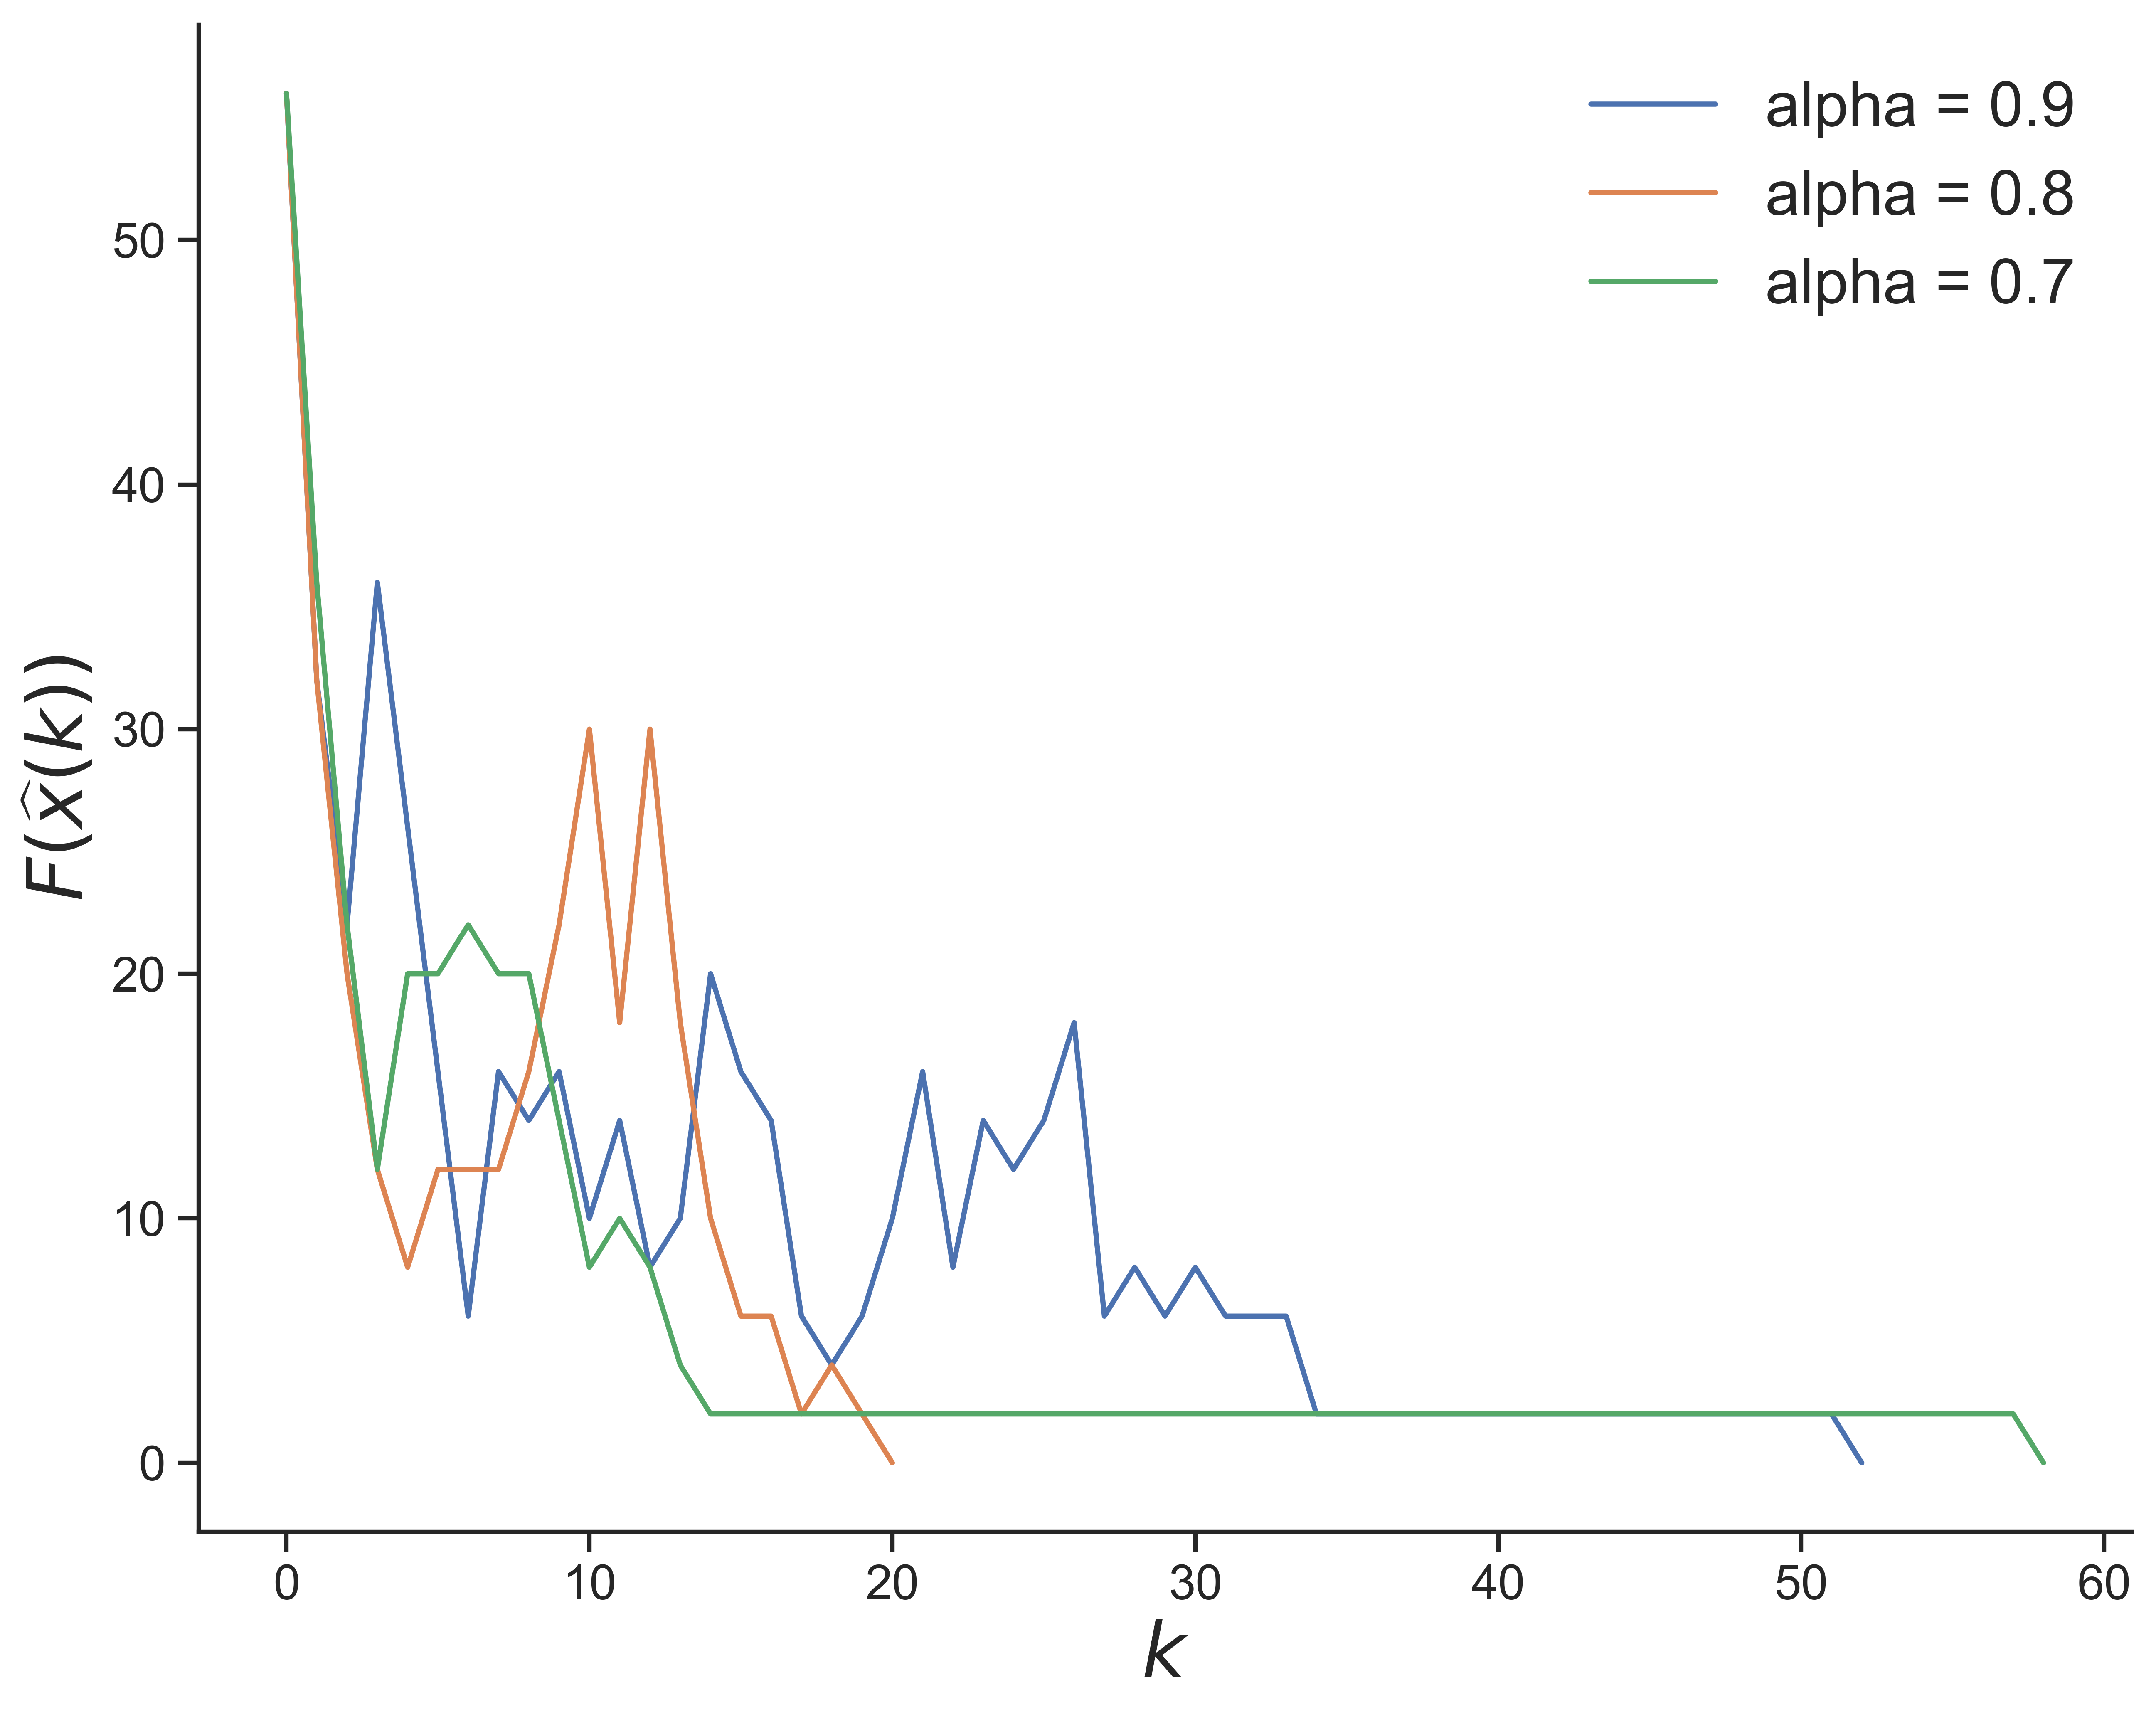
\includegraphics [width=120mm]{queens8}
\caption{ --- Оптимизация расстановки 8 ферзей  в зависимости от гиперпараметра $\alpha$.}
\label{img:queens8}
\end{figure}

\begin{figure}[h!]
\centering
\includegraphics [width=120mm]{queens25}
\caption{ --- Оптимизация расстановки 25 ферзей  в зависимости от гиперпараметра $\alpha$.}
\label{img:queens25}
\end{figure}

\newpage

%%%%%%%%%%%%%%%%%%%%%%%%%%%%%%%%%%%%%%%%%%%%%%%%%%%%%%%%


\subsection{Минимизация негладкой функции}

\noindent Воспользуемся алгоритмом имитации отжига для нахождения глобального минимума следующей функции:
\[
f(x) = x^2 (1 + |\sin 80x|).
\]

	\begin{figure}[h]
	\centering
	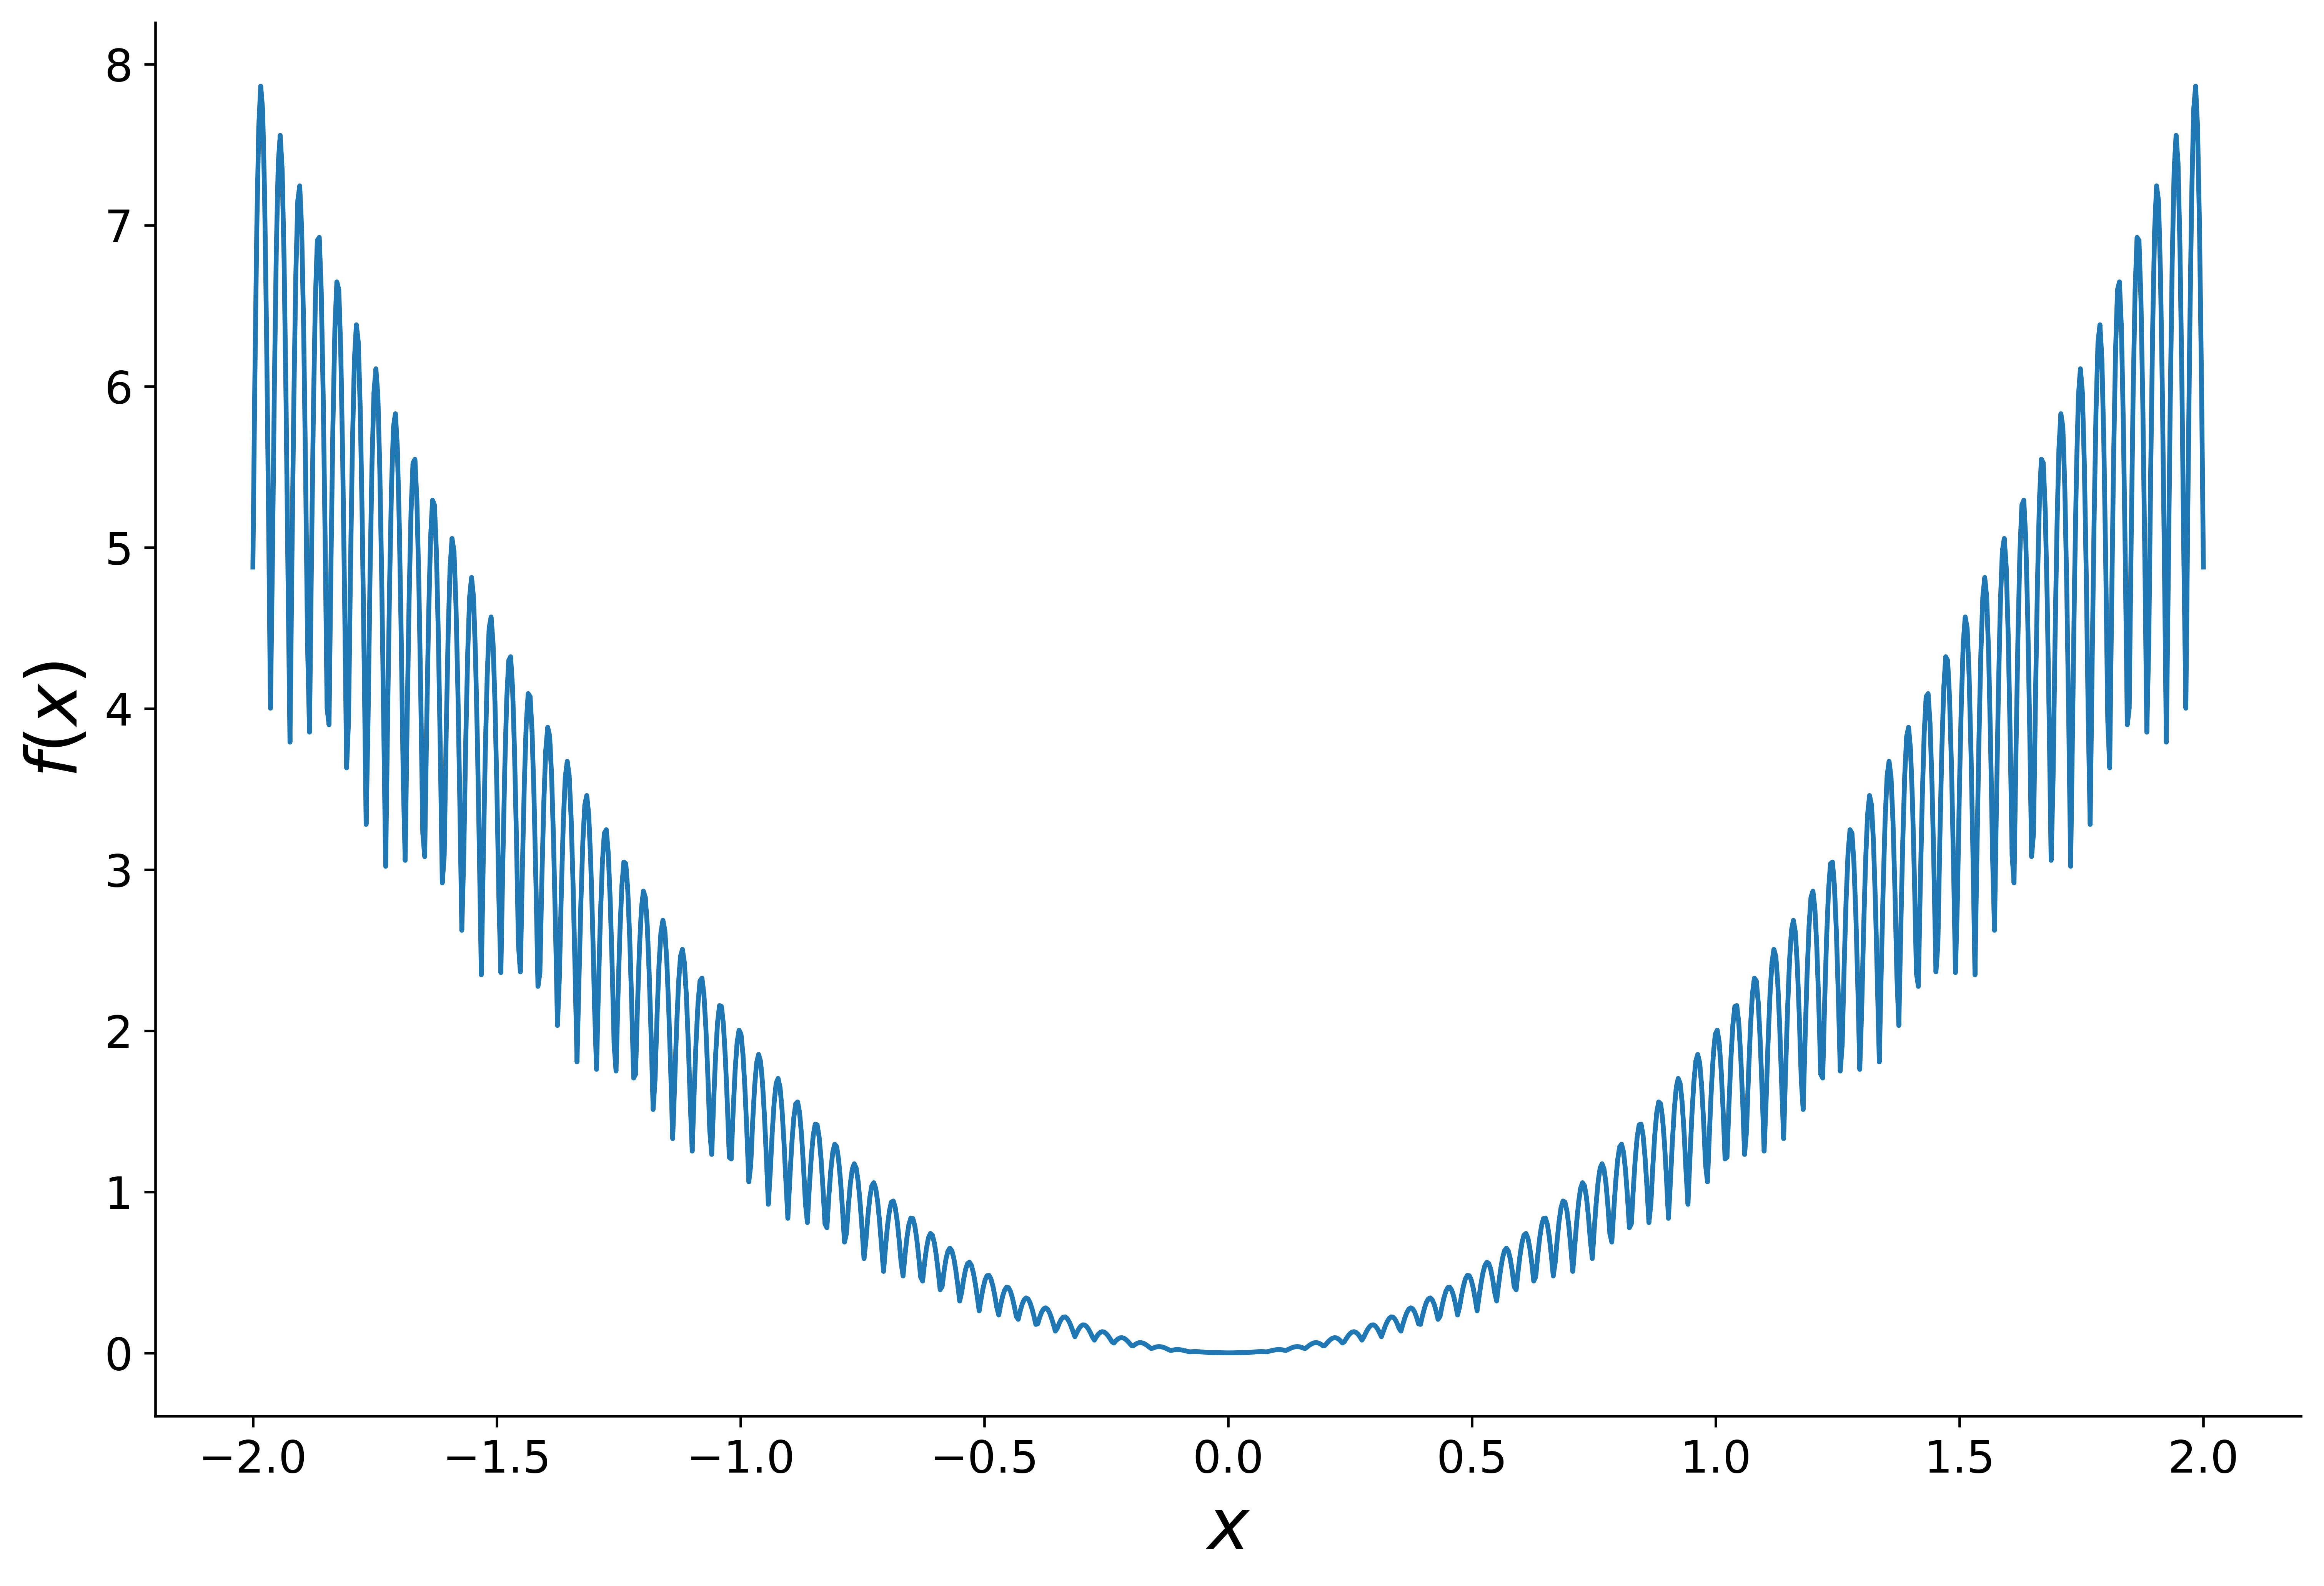
\includegraphics[width=120mm]{func_min}
	\caption{}
	\label{img:func_min}
\end{figure}

Стандартные методы оптимизации --- к примеру, метод градиентного спуска --- в данном случае не применимы. Вследствие наличия модуля этп функция не дифференцируема. Также она имеет очень большое количество локальных минимумов, что затрудняет, к примеру, мультистарт --- запуск градиентного спуска из разных начальных направлений.

Применим наш алгоритм к данной задачи. Пусть~$T(0) = 0.6$. Для понижения температуры будем использовать Больцмановский отжиг~(\ref{eq:boltzman}), а в качестве функции вероятностных распределений $G$ — семейство нормальных распределений~(\ref{eq:normal_G}).

\begin{pyin}
def SA(space, T, epsilon): # за space берется np.linspace(-2, 2, 1000)
  x_hat = np.random.choice(space)
  T_0 = T
  k = 1
  while True:
     x_tilda = np.random.normal(x_hat, T)
     delta = F(x_tilda) - F(x_hat)
     prob = np.exp(- delta / T)
     if (delta < 0) or (prob >= np.random.random()):
        x_hat = x_tilda
\end{pyin}

\begin{pyprint}
     if (x_hat < epsilon) and (x_hat > 0):
        return x_hat
     T = T_0 / np.log(1 + k)
     k += 1
\end{pyprint}

Остановка итерационного процесса и скорость метода зависят от того, насколько близко мы хотим приблизиться к глобальному минимуму. Так, при точности~$10^{-1}$, что довольно много, для 1000 повторений алгоритма метод отжига находит глобальный минимум в среднем за~1.97e-3~секунды со стандартным отклонением в~3.47e-5~секунды. Однако, увеличив точность до~$10^{-6}$, среднюю скорость занимает уже~1.27~секунды со стандартным отклонением в~2.1e-5~секунды. Это наглядно представлено на рисунке \ref{img:func_min2}.

\begin{figure}[h!]
\centering
\includegraphics[width=\linewidth]{func_min2}
\caption{ --- Оптимизационный процесс в зависимости от точности.}
\label{img:func_min2}
\end{figure}

\newpage

\subsection{Задача коммивояжера}

\noindent \textit{Задача коммивояжера} или TSP (Traveling Salesman Problem) является образцовым методом проверки многих оптимизационных алгоритмов и заключается в поиске кратчайшего маршрута между городами. Путь должен быть проложен так, чтобы маршрут единственно проходил через все города и его конечная точка совпадала с  изначальной.

TSP имеет множество приложений в планировании и логистике, а также выступает в качестве подзадачи во многих других областях.  В таком случае города могут представлять, к примеру, клиентов, а расстояние между городами — время или стоимость путешествия.

\begin{figure}[h!]
\centering
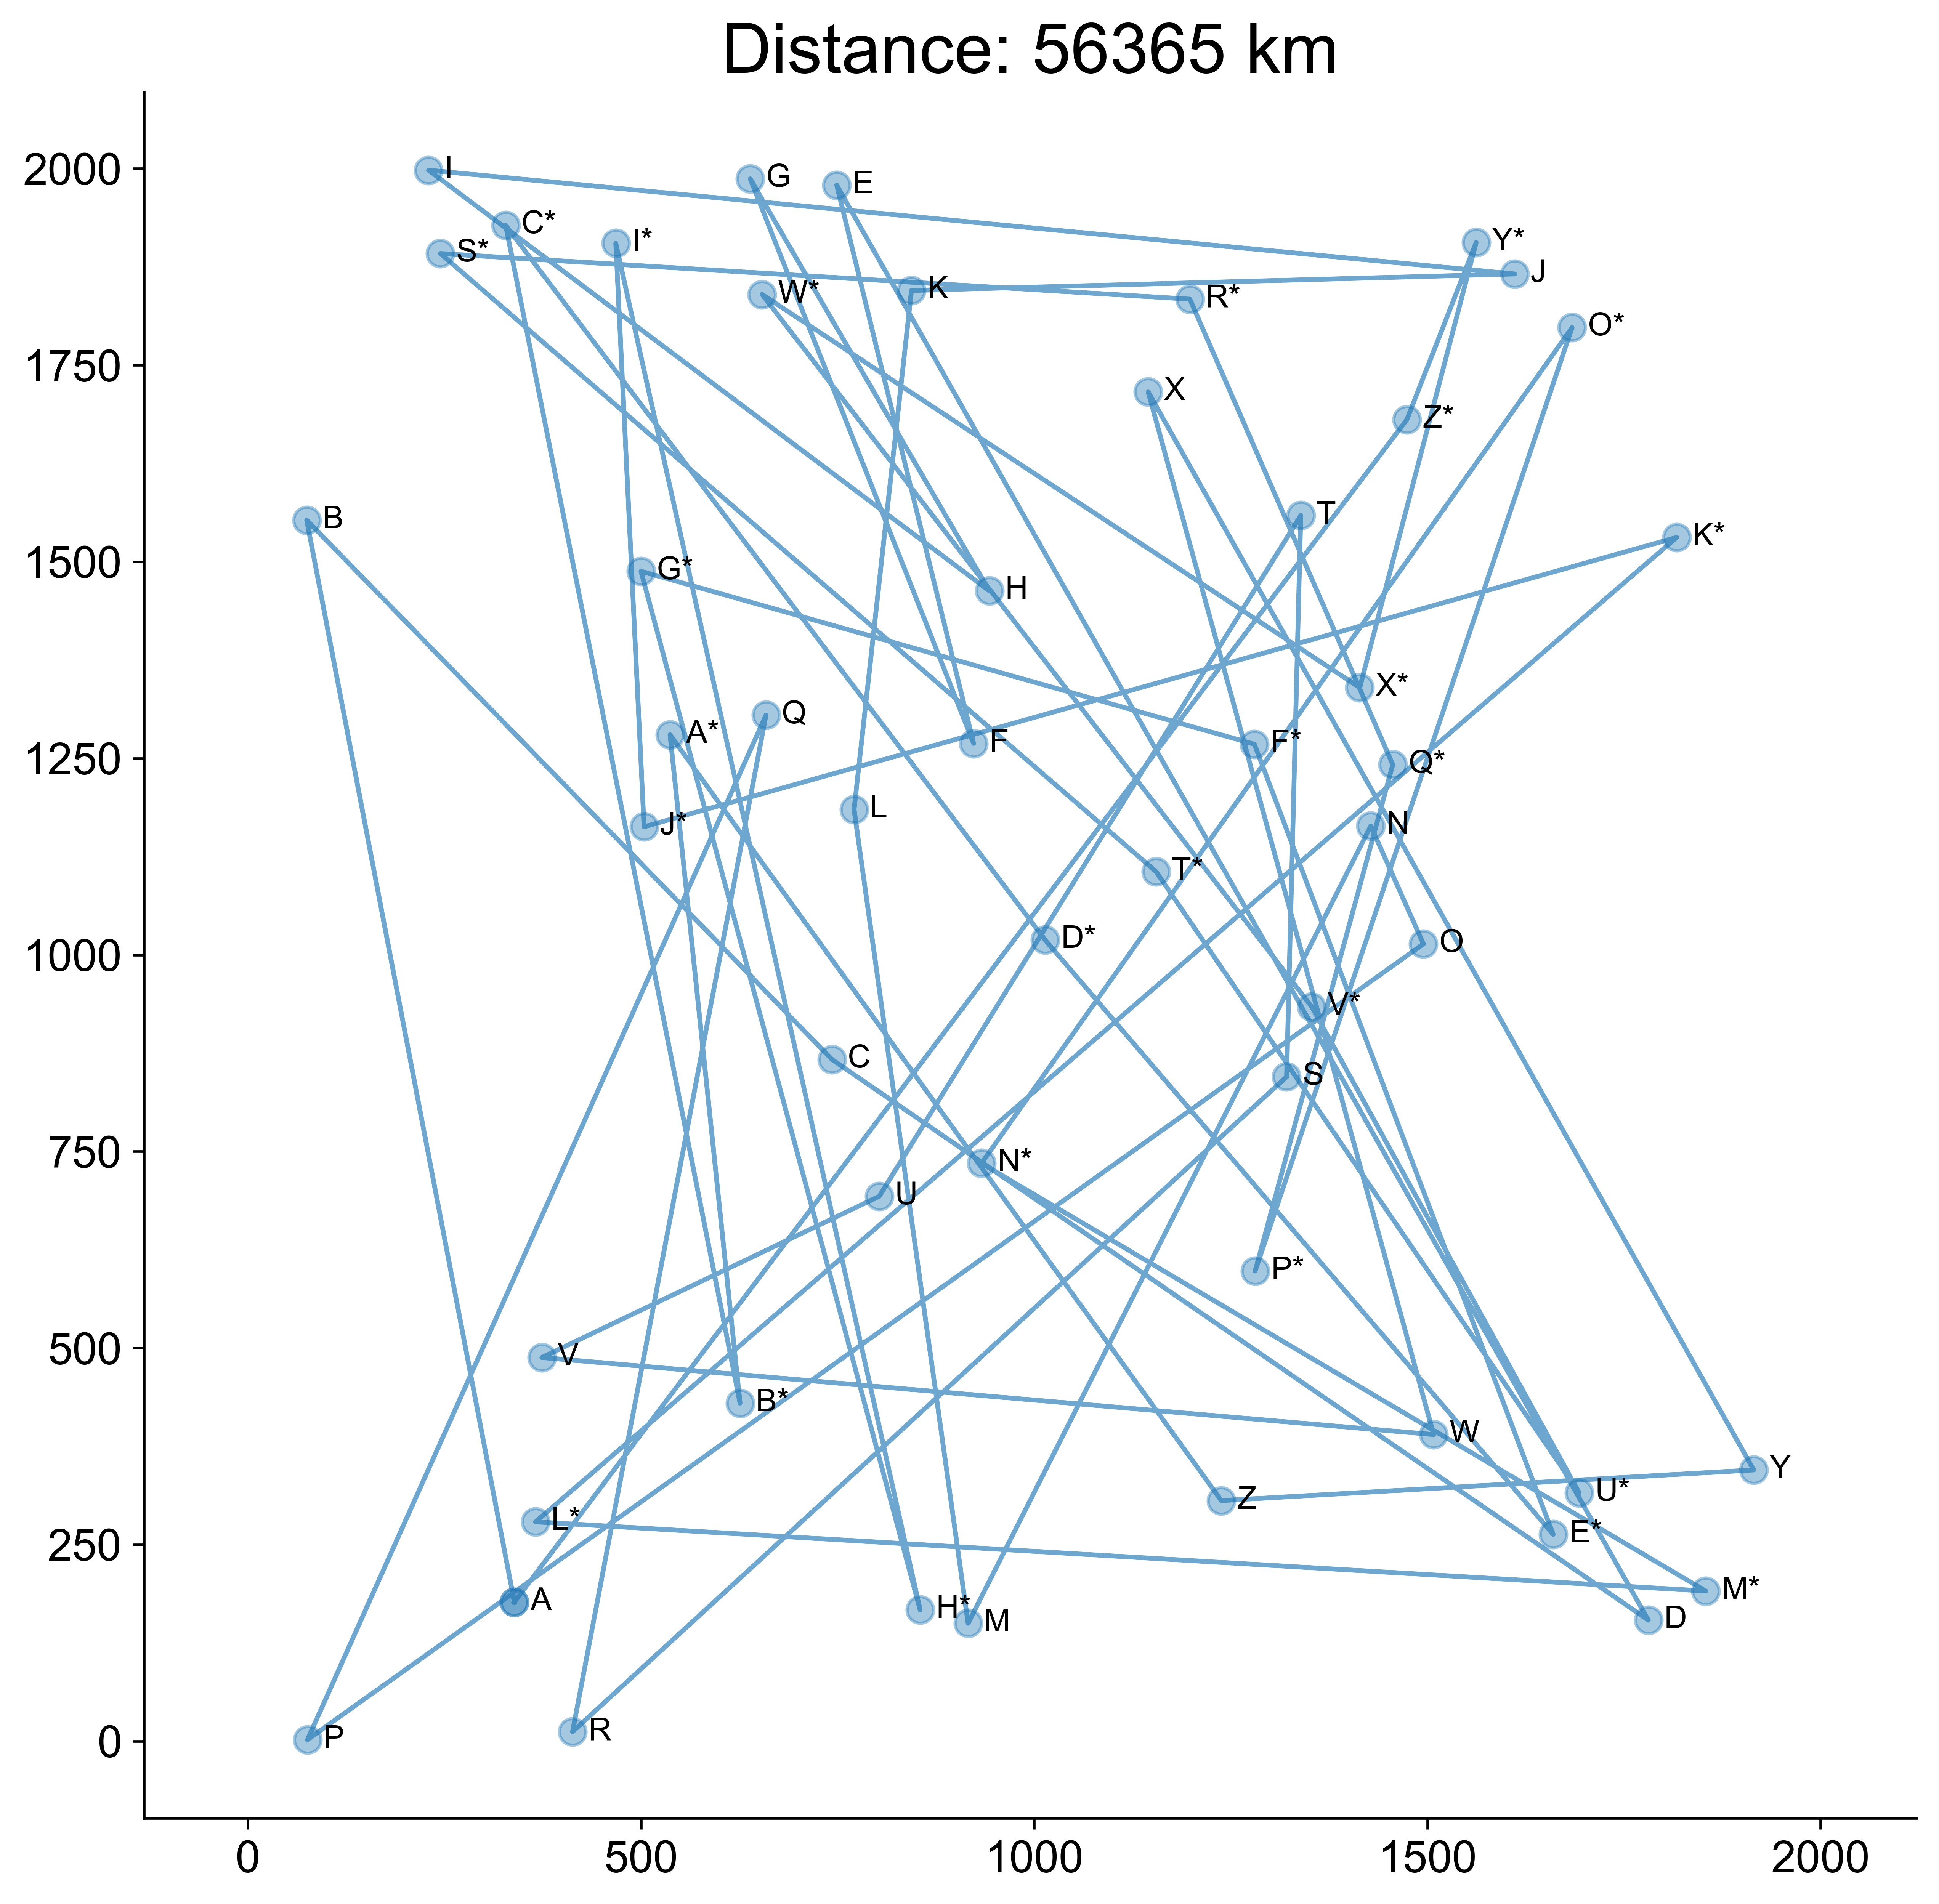
\includegraphics [width=120mm]{TSP1}
\caption{ --- Изначальный маршрут для 26-ти городов.}
\label{img:tsp1}
\end{figure}

Для нашего примера создадим карту. Функция map\_city будет принимать желаемое количество городов в качестве входных данных и выдавать два списка, из которых далее создается общий список кортежей. Первым элементом кортежа является наименование города, а вторым --- его расположение в декартовой системе координат.

\begin{pyin}
def map_city(cities_num):
  letters = [chr(i) for i in range(65, 65 + cities_num)]
  coord = np.random.randint(1, 500, size=(cities_num, 2))
  return letters, coord
\end{pyin}

Наш маршрут будет состоять из 26-ти городов.

\begin{pyin}
names, cities = map_city(26)
store_val = list(zip(names, cities))
\end{pyin}


Определим расстояние от города i до всех остальных посредством функции distance\_dict. Для измерения расстояния между городами будем использовать евклидову метрику. Напомним, что евклидово расстояние между точками~$x = (x_1, ..., x_d)$~и~$u = (u_1, ..., u_d)$~задается как:
\[
d (x, u)
=
\sqrt{
\sum_{i = 1}^d \limits
(x_i - u_i)^2
}
\]

\begin{pyin}
def distance_dict(cities, n):
  d = dict()
  for i in range(n):
     city = dict()
     for j in range(n):
        if i == j:
           continue
        c_a = cities[i][1]
        c_b = cities[j][1]
        dist = np.sqrt((c_a[0] - c_b[0]) ** 2 + (c_a[1] - c_b[1]) ** 2)
        city[cities[j][0]] = dist
     d[cities[i][0]] = city
  return d
\end{pyin}


\begin{pyin}
cities_d = distance_dict(store_val, len(store_val))
\end{pyin}


Функция F для подсчета общего расстояния путешествия:

\begin{pyin}
def F(path, cities):
  dist = 0
  for i in range(len(path) - 1):
     dist += cities[path[i]][path[i + 1]]
  dist += cities[path[i + 1]][path[0]]
  return dist
\end{pyin}

За функцию G будет выступать простая перестановка как и в задаче о N ферзях.

\begin{pyin}
def G(path, n):
  pos = path.copy()
  while True:
     i = np.random.randint(0, n - 1)
     j = np.random.randint(0, n - 1)
     if i != j:
        break
     pos[i], pos[j] = pos[j], pos[i]
  return pos
\end{pyin}

\begin{figure}[h!]
\centering
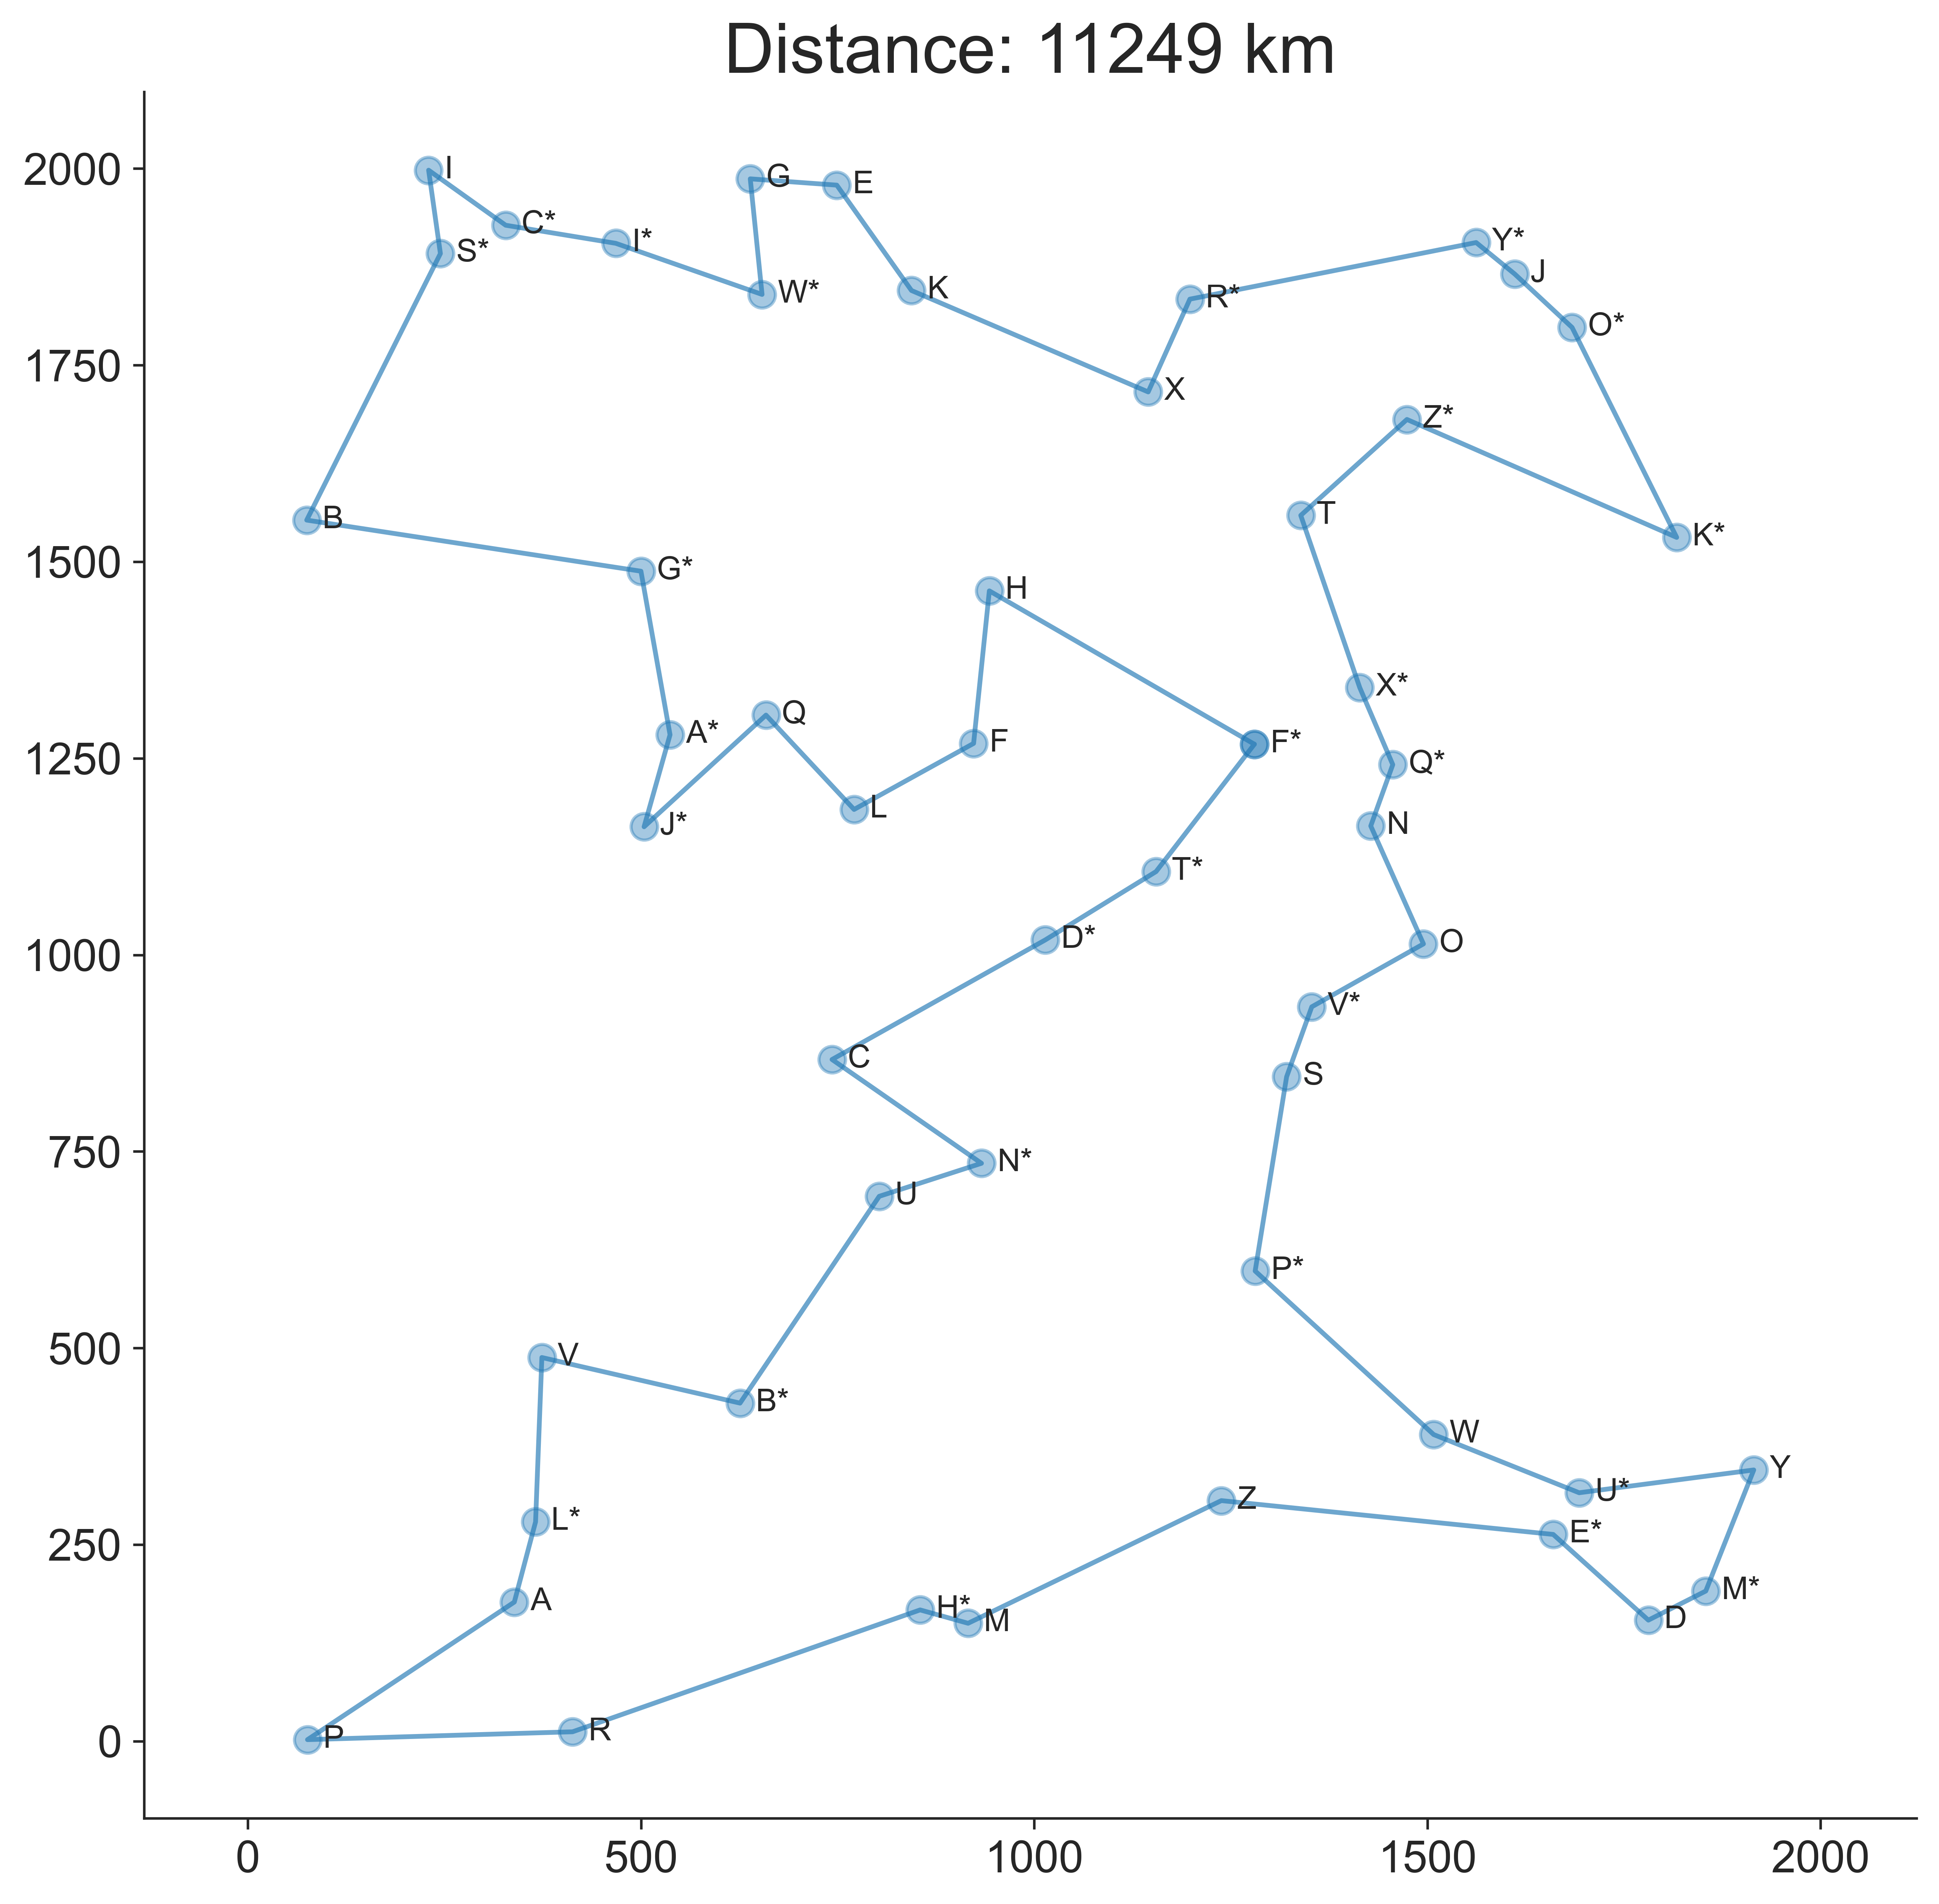
\includegraphics [width=120mm]{TSP2}
\caption{ --- Применение метода отжига для построения оптимального маршрута для 26-ти городов.}
\label{img:tsp2}
\end{figure}


Для понижения температуры используем Больцмановский отжиг~(\ref{eq:boltzman}).

\begin{pyin}
def SA(path, T):
  path_hat = path
  n = len(path_hat)
  np.random.shuffle(path_hat)
  T_0 = T
  k = 1
  for i in range(100000):
     path_tilda = G(path_hat, n)
     delta = F(path_tilda, cities_d) - F(path_hat, cities_d)
     prob = np.exp(- delta / T)
\end{pyin}

Теперь построим оптимальный маршрут (рис.~\ref{img:tsp2}).

\begin{pyin}
path_opt = SA(names, 100)
\end{pyin}

Несмотря на то, что метод отжига сократил преодалеваемую дистанцию, TSP была решена неидеально. К примеру, можно выделить соединение вершин E-S-L-V: очевидно, оно не оптимально, поскольку путь E-L-S-V имеет меньшее расстояние.

\subsection{Вывод}
